%=====================================================================
%  SOEN 6011 -- Summer 2026 -- Deliverable 2 (D2)
%  Function F5:  a * b^x
%  Author: Aafreen Fathima
%
% 
%=====================================================================
\documentclass[10pt,aspectratio=169]{beamer}

\usepackage[T1]{fontenc}
\usepackage[utf8]{inputenc}
\usepackage{amsmath,amssymb}
\usepackage{booktabs}
\usepackage{array}
\usepackage{algpseudocode}
\usepackage{listings}
\usepackage{graphicx}
\lstdefinestyle{py}{
  language=Python, basicstyle=\ttfamily\scriptsize,
  keywordstyle=\color{mDarkTeal}\bfseries, commentstyle=\color{mLightTeal}\itshape,
  stringstyle=\color{mAccent}, showstringspaces=false,
  numbers=left, numberstyle=\tiny\color{gray}, numbersep=6pt,
  breaklines=true, frame=none, xleftmargin=1.6em, aboveskip=2pt, belowskip=2pt,
}
\renewcommand{\textproc}[1]{\textbf{#1}}   % function names: bold roman (no smallcaps warning)
\newcommand{\pc}[1]{\mathrm{#1}}            % procedure call in math
\usepackage{tikz}
\usetikzlibrary{mindmap,trees,backgrounds}
\usepackage{xcolor}

% Force a clean sans-serif look everywhere (Metropolis vibe)
\renewcommand{\familydefault}{\sfdefault}
\usefonttheme{professionalfonts}

%------------------------- MetropolisLite theme ----------------------
\definecolor{mDarkTeal}{HTML}{23373B}
\definecolor{mLightTeal}{HTML}{2C5054}
\definecolor{mAccent}{HTML}{EB811B}     % orange accent
\definecolor{mFg}{HTML}{23373B}
\definecolor{mBg}{HTML}{FAFAFA}

\setbeamercolor{normal text}{fg=mFg,bg=mBg}
\setbeamercolor{alerted text}{fg=mAccent}
\setbeamercolor{frametitle}{fg=white,bg=mDarkTeal}
\setbeamercolor{title}{fg=mDarkTeal}
\setbeamercolor{structure}{fg=mDarkTeal}
\setbeamercolor{itemize item}{fg=mAccent}
\setbeamercolor{itemize subitem}{fg=mLightTeal}
\setbeamercolor{section title}{fg=white}

\setbeamertemplate{navigation symbols}{}   % no nav clutter
\setbeamertemplate{itemize items}[circle]
\setbeamertemplate{itemize subitem}{--}

% Flat frame title with a thin accent progress rule underneath
\setbeamertemplate{frametitle}{%
  \nointerlineskip
  \begin{beamercolorbox}[wd=\paperwidth,ht=3.2ex,dp=1.2ex,leftskip=0.6cm,rightskip=0.6cm]{frametitle}%
    \usebeamerfont{frametitle}\insertframetitle%
  \end{beamercolorbox}%
  \nointerlineskip
  \begin{beamercolorbox}[wd=\paperwidth,ht=0.4ex,dp=0ex]{}%
    \hspace*{-0pt}\textcolor{mAccent}{\rule{\paperwidth}{0.4ex}}%
  \end{beamercolorbox}%
}
\setbeamerfont{frametitle}{series=\bfseries,size=\large}

% Minimal footline: short title | author | page
\setbeamertemplate{footline}{%
  \leavevmode%
  \hbox{%
    \begin{beamercolorbox}[wd=.34\paperwidth,ht=2.4ex,dp=1ex,leftskip=.3cm]{frametitle}%
      \usebeamerfont{footline}\scriptsize F5: $a\cdot b^{x}$%
    \end{beamercolorbox}%
    \begin{beamercolorbox}[wd=.42\paperwidth,ht=2.4ex,dp=1ex,center]{frametitle}%
      \usebeamerfont{footline}\scriptsize SOEN 6011 -- D2%
    \end{beamercolorbox}%
    \begin{beamercolorbox}[wd=.24\paperwidth,ht=2.4ex,dp=1ex,rightskip=.3cm]{frametitle}%
      \usebeamerfont{footline}\scriptsize\hfill\insertframenumber\,/\,\inserttotalframenumber%
    \end{beamercolorbox}%
  }%
}

% Big flat section slide
\setbeamertemplate{section page}{%
  \begin{center}
    {\usebeamerfont{title}\usebeamercolor[fg]{title}\bfseries\Large\insertsection}
  \end{center}
}
%--------------------- end MetropolisLite theme ----------------------

\title{Function F5: $a\cdot b^{x}$}
\subtitle{Deliverable 2 --- Problems 5--7}
\author{Aafreen Fathima}
\institute{SOEN 6011 (Section CC) --- Software Engineering Processes\\ Summer 2026, Concordia University}
\date{July 15, 2026}

\begin{document}

%========================= TITLE ====================================
{\setbeamertemplate{footline}{}
\begin{frame}[plain]
  \vfill
  \begin{center}
    {\Large\bfseries\textcolor{mDarkTeal}{Function F5:\ \ $a\,b^{x}$}}\\[0.4em]
    \textcolor{mAccent}{\rule{0.55\textwidth}{1.2pt}}\\[0.8em]
    {\large Deliverable 2 --- Problems 5--7}\\[0.4em]
    {\small From-scratch implementation, GUI, repository \& requirements}\\[1.6em]
    \textbf{Aafreen Fathima}\\[0.3em]
    \small Student ID: 40331369\\[1.2em]
    \small SOEN 6011 (Section CC) --- Software Engineering Processes\\
    \small Summer 2026 --- Concordia University
  \end{center}
  \vfill
\end{frame}}

%===================== RECAP ========================================
\begin{frame}{Recap: F5 and the chosen approach}
  \small
  \textbf{Function.}\ \ $f(x) = a\,b^{x}$ with $b>0$; $a,b$ real constants, $x$ real variable. Models exponential growth ($b>1$) and decay ($0<b<1$).
  \vspace{0.5em}

  \textbf{Selected algorithm (D1, Problem 4).}\ \ Compute via the exp--log identity:
  \[ a\,b^{x} \;=\; a\cdot\exp\!\big(x\,\ln b\big) \]
  \vspace{0.2em}

  \textbf{This deliverable (D2).}
  \begin{itemize}\setlength\itemsep{0.2em}
    \item \textbf{Problem 5} --- reimplement \emph{from scratch} (no libraries), add a Tkinter GUI and exception handling.
    \item \textbf{Problem 6} --- public Git repository with high-quality history.
    \item \textbf{Problem 7} --- update the requirements based on what implementation revealed.
  \end{itemize}
\end{frame}

%===================== PROBLEM 5 SECTION ============================
\section{Problem 5: From-scratch Implementation}
{\setbeamercolor{background canvas}{bg=mDarkTeal}
\begin{frame}[plain]
  \vfill
  \begin{center}
    {\Large\bfseries\textcolor{white}{Problem 5 --- Implementation from Scratch}}\\[0.5em]
    \textcolor{mAccent}{\rule{0.4\textwidth}{1.0pt}}\\[0.5em]
    {\normalsize\textcolor{white!85!black}{no libraries $\cdot$ Tkinter GUI $\cdot$ exceptions --- 60 marks}}
  \end{center}
  \vfill
\end{frame}}

\begin{frame}{What ``from scratch'' means here}
  \small
  Permitted: \textbf{input, output, arithmetic, and user-interface} functions only. Everything else is hand-implemented.
  \vspace{0.5em}
  \begin{columns}[T]
    \begin{column}{0.5\textwidth}
      \textbf{Removed / re-implemented}
      \begin{itemize}\footnotesize\setlength\itemsep{0.2em}
        \item[\textcolor{mAccent}{$\times$}] \texttt{math} library
        \item[\textcolor{mAccent}{$\times$}] \texttt{**} power operator
        \item[\textcolor{mAccent}{$\times$}] \texttt{abs} $\to$ \texttt{\_abs}
        \item[\textcolor{mAccent}{$\times$}] round/int $\to$ \texttt{\_round\_to\_int}, \texttt{\_floor\_to\_int}
        \item[\textcolor{mAccent}{$\times$}] $2^{n}$ $\to$ \texttt{\_int\_pow2} (by squaring)
      \end{itemize}
    \end{column}
    \begin{column}{0.5\textwidth}
      \textbf{Kept (allowed)}
      \begin{itemize}\footnotesize\setlength\itemsep{0.2em}
        \item[\textcolor{green!50!black}{$\checkmark$}] \texttt{float()} --- input conversion
        \item[\textcolor{green!50!black}{$\checkmark$}] \texttt{.strip()} --- input parsing
        \item[\textcolor{green!50!black}{$\checkmark$}] \texttt{tkinter} --- user interface
        \item[\textcolor{green!50!black}{$\checkmark$}] $+\ -\ \times\ \div$ --- arithmetic
      \end{itemize}
    \end{column}
  \end{columns}
  \vspace{0.4em}
  \footnotesize\textcolor{mLightTeal}{Captured as a requirement in Problem 7 (REQ-C-1) so it stays verifiable.}
\end{frame}

\begin{frame}{Module structure}
  \small
  Separated into three modules so the numerical core is testable in isolation and reusable in D3.
  \vspace{0.6em}

  \begin{tabular}{@{}>{\ttfamily}p{3.4cm} >{\raggedright\arraybackslash}p{8.2cm}@{}}
    \toprule
    \normalfont\textbf{Module} & \textbf{Responsibility} \\
    \midrule
    f5\_mathcore.py & From-scratch $\ln$, $\exp$, helpers; \texttt{power\_abx}. No libraries. \\
    f5\_exceptions.py & \texttt{CalculatorError} $\rightarrow$ \texttt{DomainError}, \texttt{OverflowGuard}, \texttt{InputError}. \\
    f5\_gui.py & Tkinter interface; parses input, calls the core, shows results/errors. \\
    test\_f5\_d2.py & PyUnit suite (primitives, accuracy, guards). \\
    \bottomrule
  \end{tabular}
  \vspace{0.5em}

  \footnotesize\textcolor{mLightTeal}{Run with no IDE or build tool:\ \ \texttt{python3 f5\_gui.py}}
\end{frame}

\begin{frame}[fragile]{Core: the arithmetic primitives (from scratch)}
\begin{lstlisting}[style=py]
def _int_pow2(n):           # 2**n without the ** operator
    negative = n < 0
    if negative: n = -n
    result, base = 1.0, 2.0
    while n > 0:
        if n - (n // 2) * 2 == 1:    # n is odd
            result = result * base
        base = base * base
        n = n // 2                    # exponentiation by squaring
    return 1.0 / result if negative else result
\end{lstlisting}
  \footnotesize
  \texttt{\_abs}, \texttt{\_floor\_to\_int}, and \texttt{\_round\_to\_int} are built the same way --- only comparison and arithmetic. These replace the built-ins the series expansions depend on.
\end{frame}

\begin{frame}[fragile]{Core: computing $a\,b^{x}$}
\begin{lstlisting}[style=py]
def power_abx(a, b, x):
    if b <= 0.0:
        raise DomainError("base b must be > 0 ...")   # REQ-F-4
    if a == 0.0: return 0.0                            # REQ-F-6
    if b == 1.0: return a                              # REQ-F-6
    t = x * _ln(b)      # _ln : atanh series (from scratch)
    m = _exp(t)         # _exp: Taylor + range reduction
    result = a * m
    inf = 1e308 * 10.0
    if result == inf or result == -inf:               # REQ-R-1
        raise OverflowGuard("result too large ...")
    return result
\end{lstlisting}
  \footnotesize\textcolor{mLightTeal}{$\ln$ and $\exp$ are the D1/Problem 3 series, now dependency-free. Sign of $t$ handles decay --- one path.}
\end{frame}

\begin{frame}{Exception handling \& helpful messages}
  \small
  A small hierarchy keeps errors domain-specific instead of leaking raw Python exceptions.
  \vspace{0.4em}

  \begin{tabular}{@{}>{\ttfamily}p{2.9cm} >{\raggedright\arraybackslash}p{9.0cm}@{}}
    \toprule
    \normalfont\textbf{Exception} & \textbf{When \& message} \\
    \midrule
    DomainError & $b\le 0$: ``The base b must be greater than 0 \dots\ not a real number.'' \\
    OverflowGuard & result out of range: ``\dots too large \dots\ Try a smaller x or a base closer to 1.'' \\
    InputError & empty/non-numeric field: names the field --- ``\lq abc\rq\ is not a valid number for \lq b\rq \dots'' \\
    \bottomrule
  \end{tabular}
  \vspace{0.5em}

  \footnotesize All three subclass \texttt{CalculatorError}; the GUI catches each and shows a plain-language message in the result panel (never a crash --- REQ-R-2).
\end{frame}

\begin{frame}{Graphical user interface (Tkinter)}
  \begin{columns}[c]
    \begin{column}{0.5\textwidth}
      \centering
      \fbox{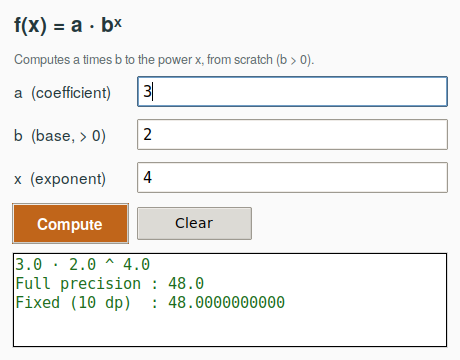
\includegraphics[width=\linewidth]{gui.png}}
    \end{column}
    \begin{column}{0.5\textwidth}
      \small
      \begin{itemize}\setlength\itemsep{0.3em}
        \item Labelled fields for $a$, $b$, $x$ \textcolor{mLightTeal}{(REQ-U-1)}
        \item \textbf{Compute} / \textbf{Clear}; \texttt{Enter} also computes
        \item Result shown in \textbf{full precision} and \textbf{fixed 10 dp} \textcolor{mLightTeal}{(REQ-P-3)}
        \item Errors appear in-panel, in red, never as a crash
        \item Standard library only; \texttt{python3 f5\_gui.py}
      \end{itemize}
      \vspace{0.3em}
      \footnotesize\textcolor{mLightTeal}{Shown: $3\cdot 2^{4}=48$.}
    \end{column}
  \end{columns}
\end{frame}

\begin{frame}{Verification}
  \small
  The from-scratch core is checked against a reference (used only in tests) with a \textbf{PyUnit} suite.
  \vspace{0.5em}
  \begin{itemize}\setlength\itemsep{0.25em}
    \item \textbf{Primitives:} \texttt{\_abs}, \texttt{\_floor\_to\_int}, \texttt{\_round\_to\_int}, \texttt{\_int\_pow2} vs.\ expected.
    \item \textbf{Accuracy:} 30{,}000 randomized inputs --- worst relative error $\approx 6.5\times10^{-14}$.
    \item \textbf{Spot values:} $3\cdot2^{4}{=}48$, $100\cdot0.5^{3}{=}12.5$, $b{=}1{\to}a$, $a{=}0{\to}0$, negative $a$.
    \item \textbf{Guards:} negative base, zero base, overflow in $\exp$ \emph{and} in the final multiply.
  \end{itemize}
  \vspace{0.4em}
  \footnotesize\texttt{\$ python3 -m unittest test\_f5\_d2 -v}\ \ $\rightarrow$\ \ \textcolor{green!50!black}{Ran 10 tests --- OK}
\end{frame}

\begin{frame}{Two bugs found by testing}
  \small
  Testing the from-scratch primitives caught two defects before submission:
  \vspace{0.5em}
  \begin{enumerate}\setlength\itemsep{0.5em}
    \item \textbf{Negative rounding.}\ \ \texttt{\_round\_to\_int(-2.6)} returned $-4$, not $-3$ --- the negative branch subtracted twice. Fixed by using \texttt{\_floor\_to\_int(v + 0.5)} for both signs.
    \item \textbf{False overflow.}\ \ An \texttt{inf} test of the form \texttt{result == result + 1.0} fired on large \emph{finite} values. Replaced with a comparison against a computed $\pm\infty$ constant.
  \end{enumerate}
  \vspace{0.3em}
  \footnotesize\textcolor{mLightTeal}{Both are now regression-covered by the test suite.}
\end{frame}

%===================== PROBLEM 6 SECTION ============================
\section{Problem 6: Version Control}
{\setbeamercolor{background canvas}{bg=mDarkTeal}
\begin{frame}[plain]
  \vfill
  \begin{center}
    {\Large\bfseries\textcolor{white}{Problem 6 --- Version Control}}\\[0.5em]
    \textcolor{mAccent}{\rule{0.4\textwidth}{1.0pt}}\\[0.5em]
    {\normalsize\textcolor{white!85!black}{public repository $\cdot$ high-quality commits --- 20 marks}}
  \end{center}
  \vfill
\end{frame}}

\begin{frame}[fragile]{Repository \& commit quality}
  \small
  \textbf{Public repository:}\\
  \texttt{\small https://github.com/aafreen-fathima/soen6011-f5-calculator}
  \vspace{0.5em}

  \textbf{README} documents the function, domain, how to run, layout, and design notes. A \texttt{.gitignore} excludes bytecode, virtualenvs, and \LaTeX\ build artifacts.
  \vspace{0.5em}

  \textbf{High-quality commits} --- imperative subject $+$ explanatory body:
\begin{lstlisting}[basicstyle=\ttfamily\scriptsize,frame=single,framesep=4pt,backgroundcolor=\color{black!5},aboveskip=3pt,belowskip=2pt]
Implement a*b^x numerical core from scratch

Compute a*b^x = a*exp(x*ln b) without the math library or the
** operator. ln uses range reduction plus an atanh series; exp
uses range reduction plus a Taylor series. Re-implement the
numeric helpers by hand: _abs, _floor_to_int, _round_to_int,
_int_pow2. Overflow guarded in exp and after the final multiply.
\end{lstlisting}
  \footnotesize\textcolor{mLightTeal}{Five commits, each scoped to one concern (exceptions, core, GUI, tests, docs).}
\end{frame}

%===================== PROBLEM 7 SECTION ============================
\section{Problem 7: Updated Requirements}
{\setbeamercolor{background canvas}{bg=mDarkTeal}
\begin{frame}[plain]
  \vfill
  \begin{center}
    {\Large\bfseries\textcolor{white}{Problem 7 --- Updated Requirements}}\\[0.5em]
    \textcolor{mAccent}{\rule{0.4\textwidth}{1.0pt}}\\[0.5em]
    {\normalsize\textcolor{white!85!black}{revised from what implementation revealed --- 20 marks}}
  \end{center}
  \vfill
\end{frame}}

\begin{frame}{What implementation revealed}
  \small
  Building the function from scratch exposed gaps in the D1 requirements:
  \vspace{0.5em}
  \begin{itemize}\setlength\itemsep{0.4em}
    \item \textbf{An unmet target.} REQ-P-2 demanded ``$\ge$15 significant digits.'' Measured worst-case error is $\sim$1e-13 (\textcolor{mAccent}{$\sim$13 digits}) --- \emph{not achievable} with these series.
    \item \textbf{A changed interface.} REQ-I-1 said ``textual''; Problem 5 mandates a \textbf{GUI}.
    \item \textbf{New obligations.} Degenerate cases, loop termination, and the from-scratch rule itself had no requirement.
  \end{itemize}
\end{frame}

\begin{frame}{Key requirement changes}
  \scriptsize
  \renewcommand{\arraystretch}{1.3}
  \begin{tabular}{@{}>{\ttfamily}p{1.5cm} p{1.5cm} >{\raggedright\arraybackslash}p{8.6cm}@{}}
    \toprule
    \normalfont\textbf{ID} & \textbf{Change} & \textbf{Detail} \\
    \midrule
    REQ-P-2 & \textcolor{mAccent}{revised} & ``$\ge$15 sig.\ digits'' $\rightarrow$ ``relative error $\le$ 1e-12'' --- verifiable, and met (tested). \\
    REQ-P-3 & \textcolor{mAccent}{revised} & Two concrete formats: full round-trip precision $+$ fixed 10 dp. \\
    REQ-I-1 & \textcolor{mAccent}{revised} & Textual UI $\rightarrow$ graphical UI (Tkinter). \\
    REQ-U-2 & \textcolor{mAccent}{revised} & Now covers empty fields as well as non-numeric; names the field. \\
    REQ-F-6 & \textcolor{green!50!black}{NEW} & $a{=}0\to0$; $b{=}1\to a$, short-circuiting before the series. \\
    REQ-R-3 & \textcolor{green!50!black}{NEW} & Each convergence loop bounded (\texttt{MAX\_ITER}) --- always terminates. \\
    REQ-C-1 & \textcolor{green!50!black}{NEW} & Core must avoid \texttt{math}, \texttt{**}, and built-in numeric helpers. \\
    \bottomrule
  \end{tabular}
  \vspace{0.5em}

  \footnotesize\textbf{Stability:} no requirement was renumbered. Revisions keep their ID; additions append (REQ-F-6, REQ-R-3, REQ-C-1). Every D1 trace reference stays valid.
\end{frame}

%===================== REFERENCES ===================================
\begin{frame}{References}
  \footnotesize
  \begin{enumerate}\setlength\itemsep{0.35em}
    \item[{[1]}] ISO/IEC/IEEE, \textit{ISO/IEC/IEEE 29148:2018 --- Systems and software engineering --- Life cycle processes --- Requirements engineering}. Geneva, Switzerland: ISO, 2018.
    \item[{[2]}] A.~Cooper, R.~Reimann, D.~Cronin, and C.~Noessel, \textit{About Face: The Essentials of Interaction Design}, 4th ed. Indianapolis, IN, USA: Wiley, 2014.
    \item[{[3]}] W.~H.~Press, S.~A.~Teukolsky, W.~T.~Vetterling, and B.~P.~Flannery, \textit{Numerical Recipes: The Art of Scientific Computing}, 3rd ed. Cambridge, U.K.: Cambridge Univ.\ Press, 2007.
    \item[{[4]}] M.~Abramowitz and I.~A.~Stegun, Eds., \textit{Handbook of Mathematical Functions}. New York, NY, USA: Dover, 1965. (Series expansions for $\ln$ and $\exp$; Newton's method.)
    \item[{[5]}] IEEE, \textit{IEEE 754-2019 --- IEEE Standard for Floating-Point Arithmetic}. New York, NY, USA: IEEE, 2019.
    \item[{[6]}] Python Software Foundation, ``tkinter --- Python interface to Tcl/Tk'' and ``unittest --- Unit testing framework,'' \textit{Python 3 Documentation}. [Online]. Available: https://docs.python.org/3/
  \end{enumerate}
  \vspace{0.3em}
  \footnotesize\textcolor{mLightTeal}{Generative-AI assistance is documented per problem on the CASTROFF slides; all wording and code are my own.}
\end{frame}

%===================== CLOSE ========================================
\begin{frame}{Summary}
  \small
  \begin{itemize}\setlength\itemsep{0.35em}
    \item \textbf{Problem 5} --- $a\,b^{x}$ reimplemented from scratch (no libraries, no \texttt{**}), with a Tkinter GUI and a custom exception hierarchy giving helpful messages. Verified: 10 PyUnit tests, worst error $\sim$6.5e-14.
    \item \textbf{Problem 6} --- public Git repository, README, and five scoped, high-quality commits.
    \item \textbf{Problem 7} --- requirements revised against the implementation: an unmet precision target made testable, the interface updated to GUI, and three new requirements added --- with stable identifiers.
  \end{itemize}
  \vspace{0.6em}
  \centering\textcolor{mDarkTeal}{\textbf{Thank you --- questions?}}
\end{frame}

\end{document}
